\documentclass[landscape]{article}
\usepackage{tikz}
\usepackage{times}
\usepackage[paperwidth=34.5cm,paperheight=15.7cm,hmargin=0.2cm,vmargin=0.5cm]{geometry}
\usepackage{ifthen}
\usetikzlibrary{matrix}
\usetikzlibrary{decorations.pathreplacing}
\usetikzlibrary{arrows}

\usepackage{pifont}% http://ctan.org/pkg/pifont
\newcommand{\cmark}{\ding{51}}%
\newcommand{\xmark}{\ding{55}}%

\begin{document}

% for double arrows a la chef
% adapt line thickness and line width, if needed
\tikzstyle{vecArrow} = [thick, line width=2pt, decoration={markings,mark=at position
   1 with {\arrow[semithick, line width=2pt]{open triangle 90}}},
   double distance=3.4pt, shorten >= 5.5pt,
   preaction = {decorate},
   postaction = {draw,line width=3.4pt, white,shorten >= 4.5pt}]
   
\tikzstyle{innerWhite} = [semithick, white,line width=1.4pt, shorten >= 4.5pt]

\begin{tikzpicture}

\tikzstyle{every node}=[font=\Large]

\pgfmathsetmacro{\x}{0}
\pgfmathsetmacro{\y}{0}

\pgfmathsetmacro{\imsizex}{8}
\pgfmathsetmacro{\imsizey}{2}

\pgfmathsetmacro{\cnnsizex}{2}
\pgfmathsetmacro{\cnnsizey}{2}

\pgfmathsetmacro{\linesize}{1}
\pgfmathsetmacro{\offset}{2}

\pgfmathsetmacro{\classify}{0.6}

\definecolor{cnnfill}{RGB}{0,0,0}
\definecolor{cnnline}{RGB}{0,0,0}

\definecolor{convfill}{RGB}{255,255,255}
\definecolor{convline}{RGB}{0,0,0}

% input image
\node[inner sep=0pt,cm={0.4 ,0.5 ,0 ,1  ,(0 cm,0 cm)}] (image) at (\x, \y)
    {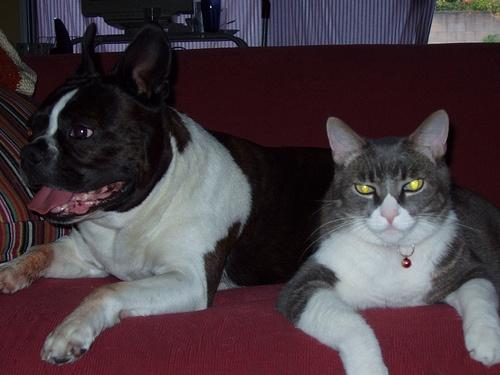
\includegraphics[width=\imsizex cm]{images/2007_001763}};
\node (image) at (\x+0.9,\y) {}; 

% CNN
\pgfmathsetmacro{\x}{\x+2.4}

\draw[convline,fill=none, dashed, line width=\linesize pt] (\x-0.55,3.6) -- ++(7.6,0) -- ++(0,-7.2) -- ++(-7.6,0) -- cycle;
\node at (\x+3.5, -3.2) {FCN: ResNet-101};


\pgfmathsetmacro{\offsetcnn}{0.12}
\pgfmathsetmacro{\offsetcnnblock}{0.08}

% orientation
\pgfmathsetmacro{\xx}{0.5}

\pgfmathsetmacro{\cubex}{0.06}
\pgfmathsetmacro{\cubey}{7}
\pgfmathsetmacro{\cubez}{8}

\pgfmathsetmacro{\multx}{0.8}
\pgfmathsetmacro{\divyz}{1.45}


%% conv1
\pgfmathsetmacro{\cubey}{\cubey/\divyz}
\pgfmathsetmacro{\cubez}{\cubez/\divyz}
\pgfmathsetmacro{\x}{\x + \cubex + \offsetcnn+0.3}
\pgfmathsetmacro{\xx}{\xx/\divyz}
\draw[convline,fill=convfill] (\x+\xx/2,\cubey/2,\cubez/2) -- ++(-\cubex,0,0) -- ++(0,-\cubey,0) -- ++(\cubex,0,0) -- cycle;
\draw[convline,fill=convfill] (\x+\xx/2,\cubey/2,\cubez/2) -- ++(0-\xx,0,-\cubez) -- ++(0,-\cubey,0) -- ++(0+\xx,0,\cubez) -- cycle;
\draw[convline,fill=convfill] (\x+\xx/2,\cubey/2,\cubez/2) -- ++(-\cubex,0,0) -- ++(0-\xx,0,-\cubez) -- ++(\cubex,0,0) -- cycle;

% pool1
\pgfmathsetmacro{\cubey}{\cubey/\divyz}
\pgfmathsetmacro{\cubez}{\cubez/\divyz}
\pgfmathsetmacro{\x}{\x + \cubex + \offsetcnn}
\pgfmathsetmacro{\xx}{\xx/\divyz}

\pgfmathsetmacro{\cubex}{\cubex * 2.5 * \multx}

%% conv2
\foreach \i in {1,...,3}
{
  \pgfmathsetmacro{\x}{\x + \i*(\cubex + \offsetcnnblock)}
  \draw[convline,fill=convfill] (\x+\xx/2,\cubey/2,\cubez/2) -- ++(-\cubex,0,0) -- ++(0,-\cubey,0) -- ++(\cubex,0,0) -- cycle;
  \draw[convline,fill=convfill] (\x+\xx/2,\cubey/2,\cubez/2) -- ++(0-\xx,0,-\cubez) -- ++(0,-\cubey,0) -- ++(0+\xx,0,\cubez) -- cycle;
  \draw[convline,fill=convfill] (\x+\xx/2,\cubey/2,\cubez/2) -- ++(-\cubex,0,0) -- ++(0-\xx,0,-\cubez) -- ++(\cubex,0,0) -- cycle;
}

%% conv3
\pgfmathsetmacro{\x}{\x + 3*(\cubex + \offsetcnnblock) + \offsetcnn}
\pgfmathsetmacro{\cubey}{\cubey/\divyz}
\pgfmathsetmacro{\cubez}{\cubez/\divyz}
\pgfmathsetmacro{\cubex}{\cubex * 2 * \multx}
\pgfmathsetmacro{\xx}{\xx/\divyz}
\foreach \i in {1,...,4}
{
  \pgfmathsetmacro{\x}{\x + \i*(\cubex + \offsetcnnblock)}
  \ifthenelse{\i=0}{
    \draw[convline,fill=convfill,densely dashed] (\x+\xx/2,\cubey/2,\cubez/2) -- ++(-\cubex,0,0) -- ++(0,-\cubey,0) -- ++(\cubex,0,0) -- cycle;
    \draw[convline,fill=convfill,densely dashed] (\x+\xx/2,\cubey/2,\cubez/2) -- ++(0-\xx,0,-\cubez) -- ++(0,-\cubey,0) -- ++(0+\xx,0,\cubez) -- cycle;
    \draw[convline,fill=convfill,densely dashed] (\x+\xx/2,\cubey/2,\cubez/2) -- ++(-\cubex,0,0) -- ++(0-\xx,0,-\cubez) -- ++(\cubex,0,0) -- cycle;
    }
    {
    \draw[convline,fill=convfill] (\x+\xx/2,\cubey/2,\cubez/2) -- ++(-\cubex,0,0) -- ++(0,-\cubey,0) -- ++(\cubex,0,0) -- cycle;
    \draw[convline,fill=convfill] (\x+\xx/2,\cubey/2,\cubez/2) -- ++(0-\xx,0,-\cubez) -- ++(0,-\cubey,0) -- ++(0+\xx,0,\cubez) -- cycle;
    \draw[convline,fill=convfill] (\x+\xx/2,\cubey/2,\cubez/2) -- ++(-\cubex,0,0) -- ++(0-\xx,0,-\cubez) -- ++(\cubex,0,0) -- cycle;
    };
}

%% conv4
\pgfmathsetmacro{\x}{\x + 4*(\cubex + \offsetcnnblock) + \offsetcnn}
\pgfmathsetmacro{\cubey}{\cubey/\divyz}
\pgfmathsetmacro{\cubez}{\cubez/\divyz}
\pgfmathsetmacro{\cubex}{\cubex * 2 * \multx}
\pgfmathsetmacro{\xx}{\xx/\divyz}
\foreach \i in {1,...,6}
{
  \pgfmathsetmacro{\x}{\x + \i*(\cubex + \offsetcnnblock)};
  \ifthenelse{\i=3 \OR \i=4}{
    \ifthenelse{\i=3}{
    \node[text width=1cm] at (\x+\cubex-0.05,0) {...};
    }
    {};
  }
  {
    \ifthenelse{\i=0}{
      \draw[convline,fill=convfill,densely dashed] (\x+\xx/2,\cubey/2,\cubez/2) -- ++(-\cubex,0,0) -- ++(0,-\cubey,0) -- ++(\cubex,0,0) -- cycle;
      \draw[convline,fill=convfill,densely dashed] (\x+\xx/2,\cubey/2,\cubez/2) -- ++(0-\xx,0,-\cubez) -- ++(0,-\cubey,0) -- ++(0+\xx,0,\cubez) -- cycle;
      \draw[convline,fill=convfill,densely dashed] (\x+\xx/2,\cubey/2,\cubez/2) -- ++(-\cubex,0,0) -- ++(0-\xx,0,-\cubez) -- ++(\cubex,0,0) -- cycle;
      }
      {
      \draw[convline,fill=convfill] (\x+\xx/2,\cubey/2,\cubez/2) -- ++(-\cubex,0,0) -- ++(0,-\cubey,0) -- ++(\cubex,0,0) -- cycle;
      \draw[convline,fill=convfill] (\x+\xx/2,\cubey/2,\cubez/2) -- ++(0-\xx,0,-\cubez) -- ++(0,-\cubey,0) -- ++(0+\xx,0,\cubez) -- cycle;
      \draw[convline,fill=convfill] (\x+\xx/2,\cubey/2,\cubez/2) -- ++(-\cubex,0,0) -- ++(0-\xx,0,-\cubez) -- ++(\cubex,0,0) -- cycle;
      };
    };
}


%% conv5
\pgfmathsetmacro{\x}{\x + 6*(\cubex + \offsetcnnblock) + \offsetcnn}
\pgfmathsetmacro{\cubey}{\cubey/\divyz}
\pgfmathsetmacro{\cubez}{\cubez/\divyz}
\pgfmathsetmacro{\cubex}{\cubex * 2 * \multx}
\pgfmathsetmacro{\xx}{\xx/\divyz}
\foreach \i in {1,...,3}
{
  \pgfmathsetmacro{\x}{\x + \i*(\cubex + \offsetcnnblock)}
  \ifthenelse{\i=0}{
    \draw[convline,fill=convfill,densely dashed] (\x+\xx/2,\cubey/2,\cubez/2) -- ++(-\cubex,0,0) -- ++(0,-\cubey,0) -- ++(\cubex,0,0) -- cycle;
    \draw[convline,fill=convfill,densely dashed] (\x+\xx/2,\cubey/2,\cubez/2) -- ++(0-\xx,0,-\cubez) -- ++(0,-\cubey,0) -- ++(0+\xx,0,\cubez) -- cycle;
    \draw[convline,fill=convfill,densely dashed] (\x+\xx/2,\cubey/2,\cubez/2) -- ++(-\cubex,0,0) -- ++(0-\xx,0,-\cubez) -- ++(\cubex,0,0) -- cycle;
    }
    {
    \draw[convline,fill=convfill] (\x+\xx/2,\cubey/2,\cubez/2) -- ++(-\cubex,0,0) -- ++(0,-\cubey,0) -- ++(\cubex,0,0) -- cycle;
    \draw[convline,fill=convfill] (\x+\xx/2,\cubey/2,\cubez/2) -- ++(0-\xx,0,-\cubez) -- ++(0,-\cubey,0) -- ++(0+\xx,0,\cubez) -- cycle;
    \draw[convline,fill=convfill] (\x+\xx/2,\cubey/2,\cubez/2) -- ++(-\cubex,0,0) -- ++(0-\xx,0,-\cubez) -- ++(\cubex,0,0) -- cycle;
    };
}
\pgfmathsetmacro{\x}{\x + 3*(\cubex + \offsetcnnblock) + \offsetcnn}
\node (cnn_output) at (\x+0.2,\y) {}; % invisible node


\pgfmathsetmacro{\x}{\x+\offset+0.9}

\node[text width=2cm] at (\x-1.5,\y) {\textbf{WSL transfer}};

\node (multimap_input) at (\x-0.7,\y) {}; % invisible node
\draw[->, line width=\linesize pt] (cnn_output) edge (multimap_input);

\pgfmathsetmacro{\mapsizex}{3}
\pgfmathsetmacro{\mapx}{0.7}
\pgfmathsetmacro{\mapy}{4}
\pgfmathsetmacro{\offsety}{0.8}
\pgfmathsetmacro{\mapr}{0.4}

\draw [decorate,decoration={brace,amplitude=12pt,mirror,raise=4pt},yshift=0pt, line width=\linesize pt] (\x,\y+1.6*\mapy+\offsety) -- (\x,\y-1.6*\mapy-\offsety) node {};

\pgfmathsetmacro{\x}{\x+1.5}
\pgfmathsetmacro{\y}{\y+0.4}

\draw[convline,fill=none, line width=\linesize pt, dashed] (\x-0.8,\y+1.5*\mapy+0.2) -- ++(3,0) -- ++(0,-13.7) -- ++(-3,0) -- cycle;
\node at (\x+0.7,\y+1.5*\mapy+0.5) {\textbf{multi-map}};

\draw[convline,fill=none, line width=\linesize pt, dotted] (\x-1.5,\y+1.5*\mapy) -- ++(7.7,0) -- ++(0,-4) -- ++(-7.7,0) -- cycle;
\node[rotate=90] at (\x-1.2,\y+\mapy) {\texttt{cat}};

\draw[convline,fill=none, line width=\linesize pt, dotted] (\x-1.5,\y+0.5*\mapy) -- ++(7.7,0) -- ++(0,-4) -- ++(-7.7,0) -- cycle;
\node[rotate=90] at (\x-1.2,\y) {\texttt{dog}};

\node[rotate=90] at (\x-1.2,\y-\mapy/2-0.35) {\ldots};

\draw[convline,fill=none, line width=\linesize pt, dotted] (\x-1.5,\y-0.5*\mapy-\offsety) -- ++(7.7,0) -- ++(0,-4) -- ++(-7.7,0) -- cycle;
\node[rotate=90] at (\x-1.2,\y-\mapy-\offsety) {\texttt{bus}};

\node[inner sep=0pt,cm={\mapr ,0.5 ,0 ,1  ,(0 cm,0 cm)}] at (\x, \y) {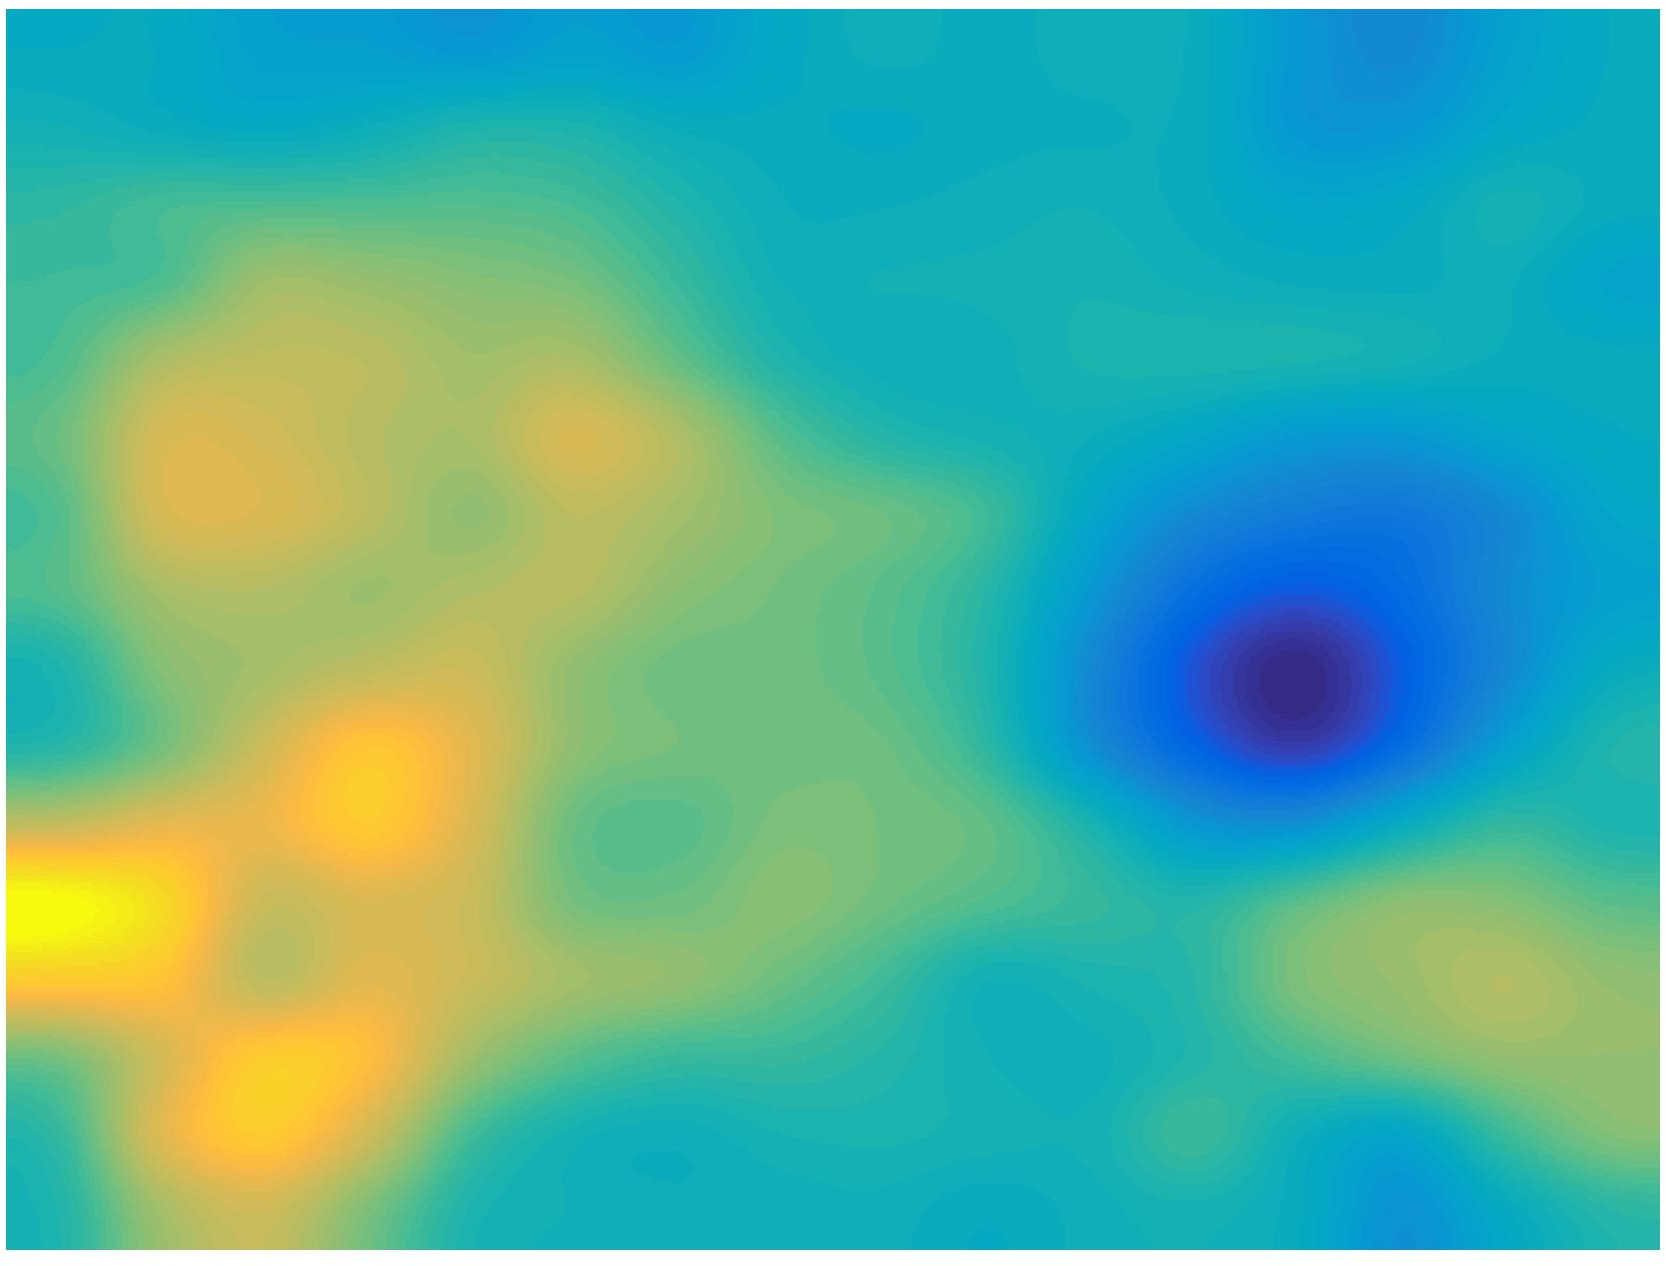
\includegraphics[width=\mapsizex cm]{images/2007_001763_dog_2}};
\node (mapi_input) at (\x-0.5,\y) {}; % invisible node

\node[inner sep=0pt,cm={\mapr ,0.5 ,0 ,1  ,(0 cm,0 cm)}] at (\x, \y+\mapy) {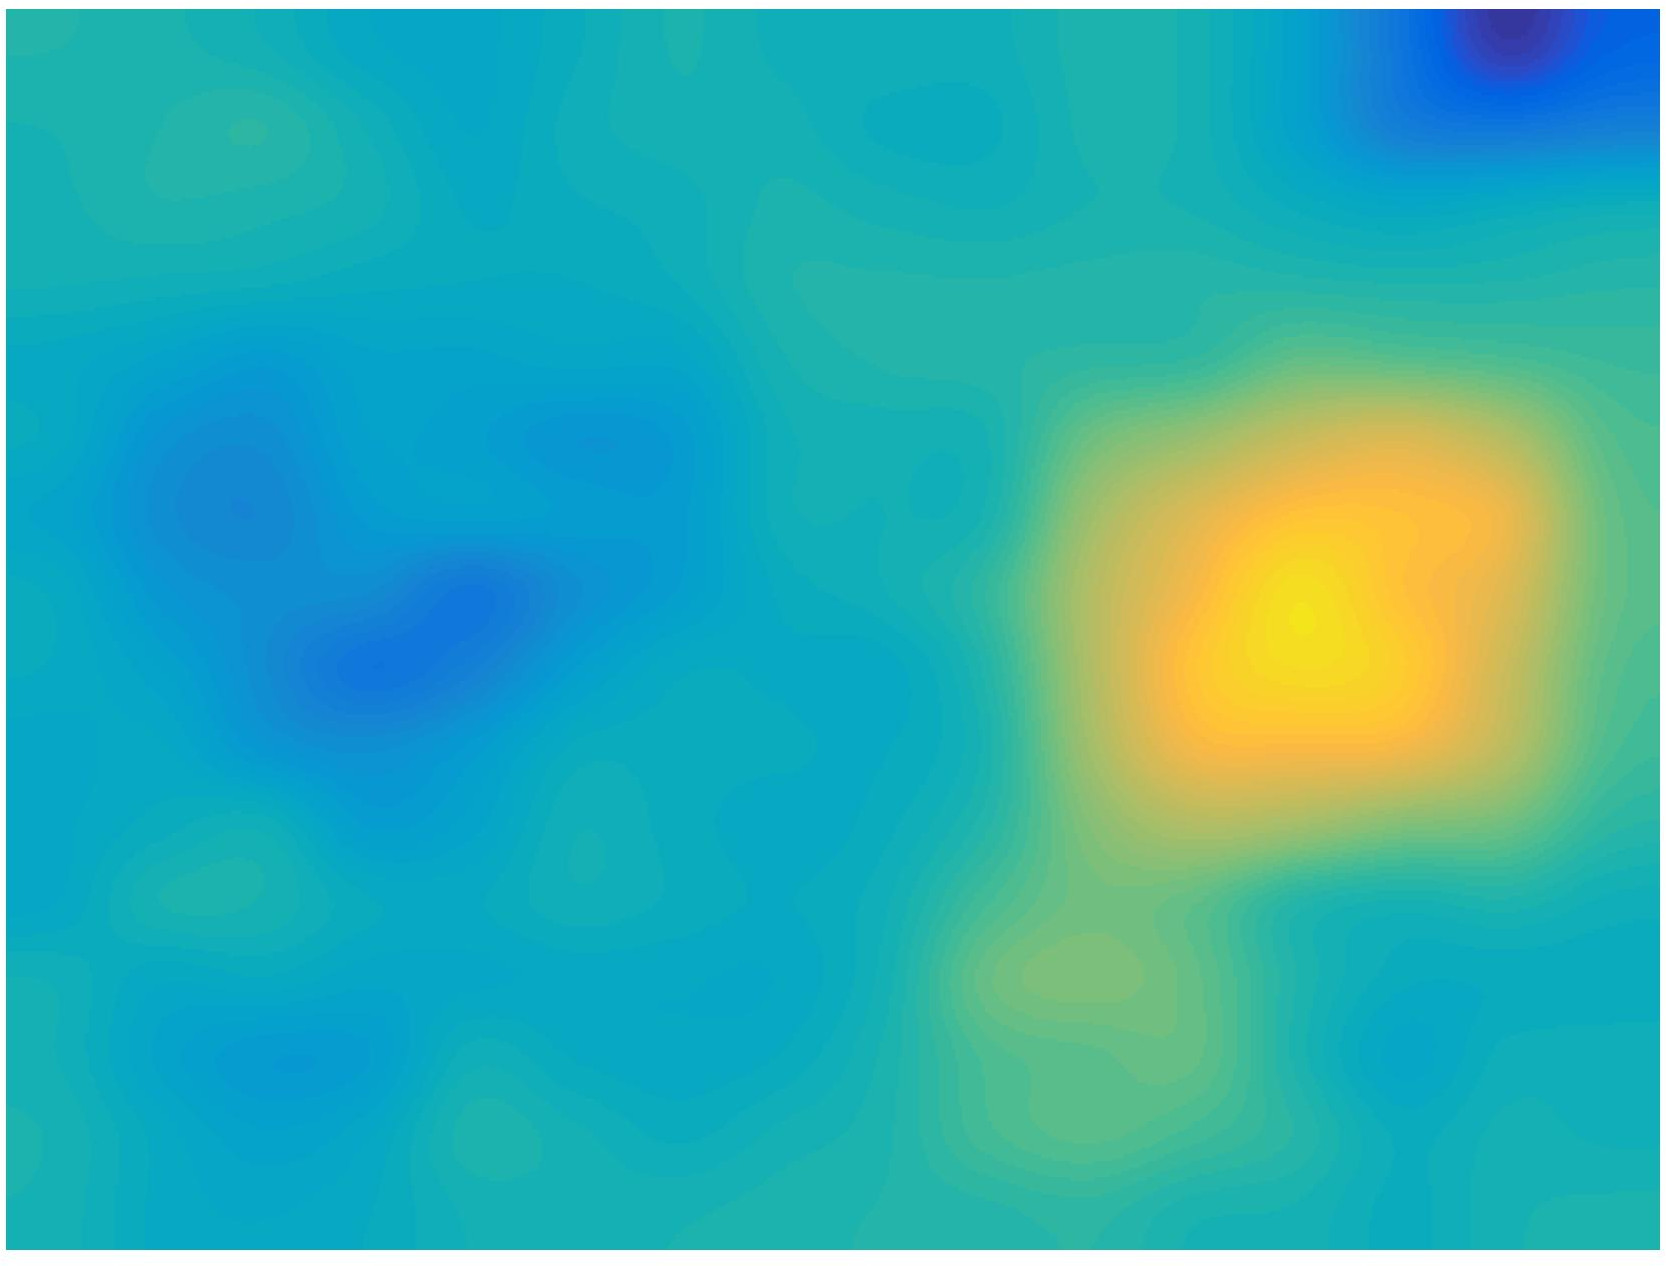
\includegraphics[width=\mapsizex cm]{images/2007_001763_cat_4}};
\node (map1_input) at (\x-0.5,\y+3) {}; % invisible node

\node[inner sep=0pt,cm={\mapr ,0.5 ,0 ,1  ,(0 cm,0 cm)}] at (\x, \y-\mapy-\offsety) {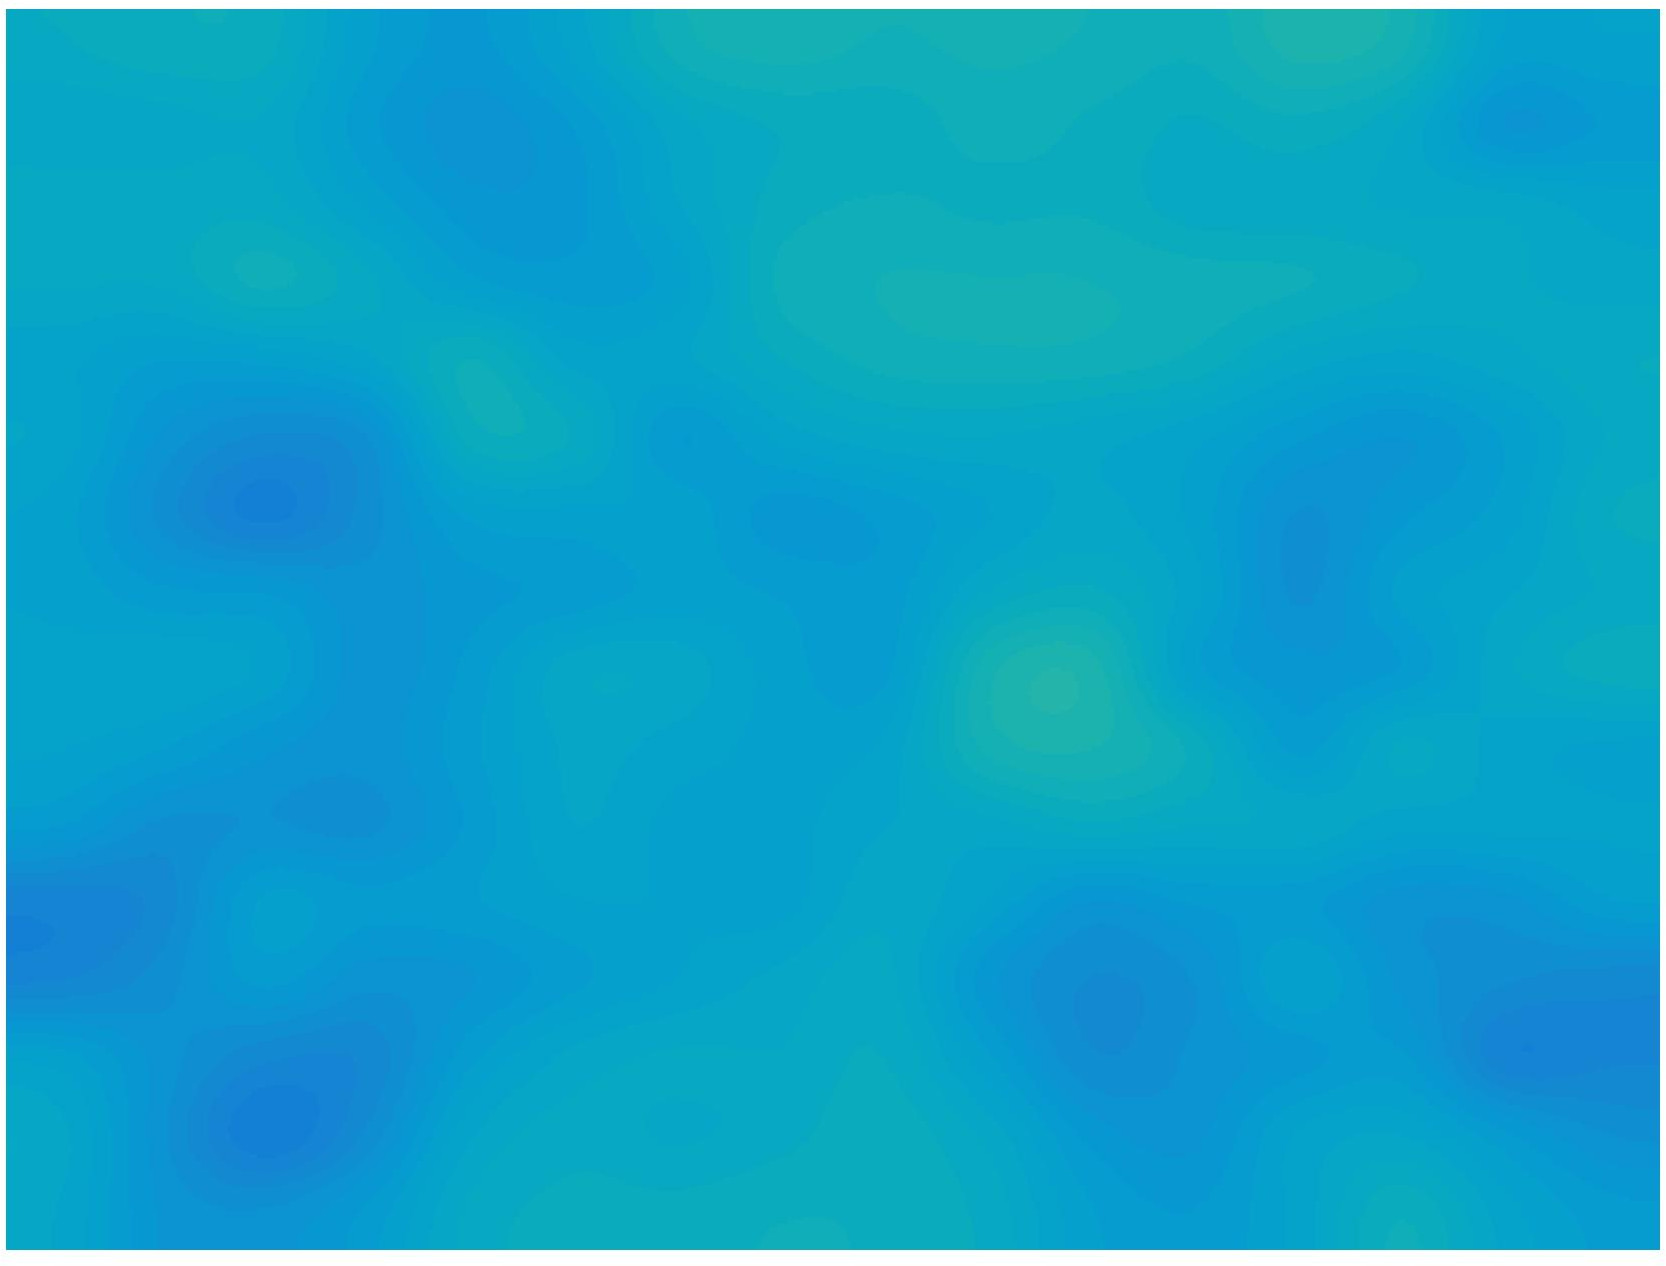
\includegraphics[width=\mapsizex cm]{images/2007_001763_train_2}};
\node (map3_input) at (\x-0.5,\y-3-\offsety) {}; % invisible node

\node at (\x+0.2,\y+\mapy-1.7) {$\ldots$};
\node at (\x+0.2,\y-1.7) {$\ldots$};
\node at (\x+0.2,\y-\mapy-1.7-\offsety) {$\ldots$};

\draw [decorate,decoration={brace,amplitude=5pt,mirror,raise=4pt}, line width=\linesize pt] (\x-0.6,\y-\mapy-1.8-\offsety) -- (\x+0.9,\y-\mapy-1.8-\offsety);
\node at (\x+0.1,\y-\mapy-2.4-\offsety) {$M$};

 
\pgfmathsetmacro{\x}{\x+2*\mapx}
\node[inner sep=0pt,cm={\mapr ,0.5 ,0 ,1  ,(0 cm,0 cm)}] at (\x, \y) {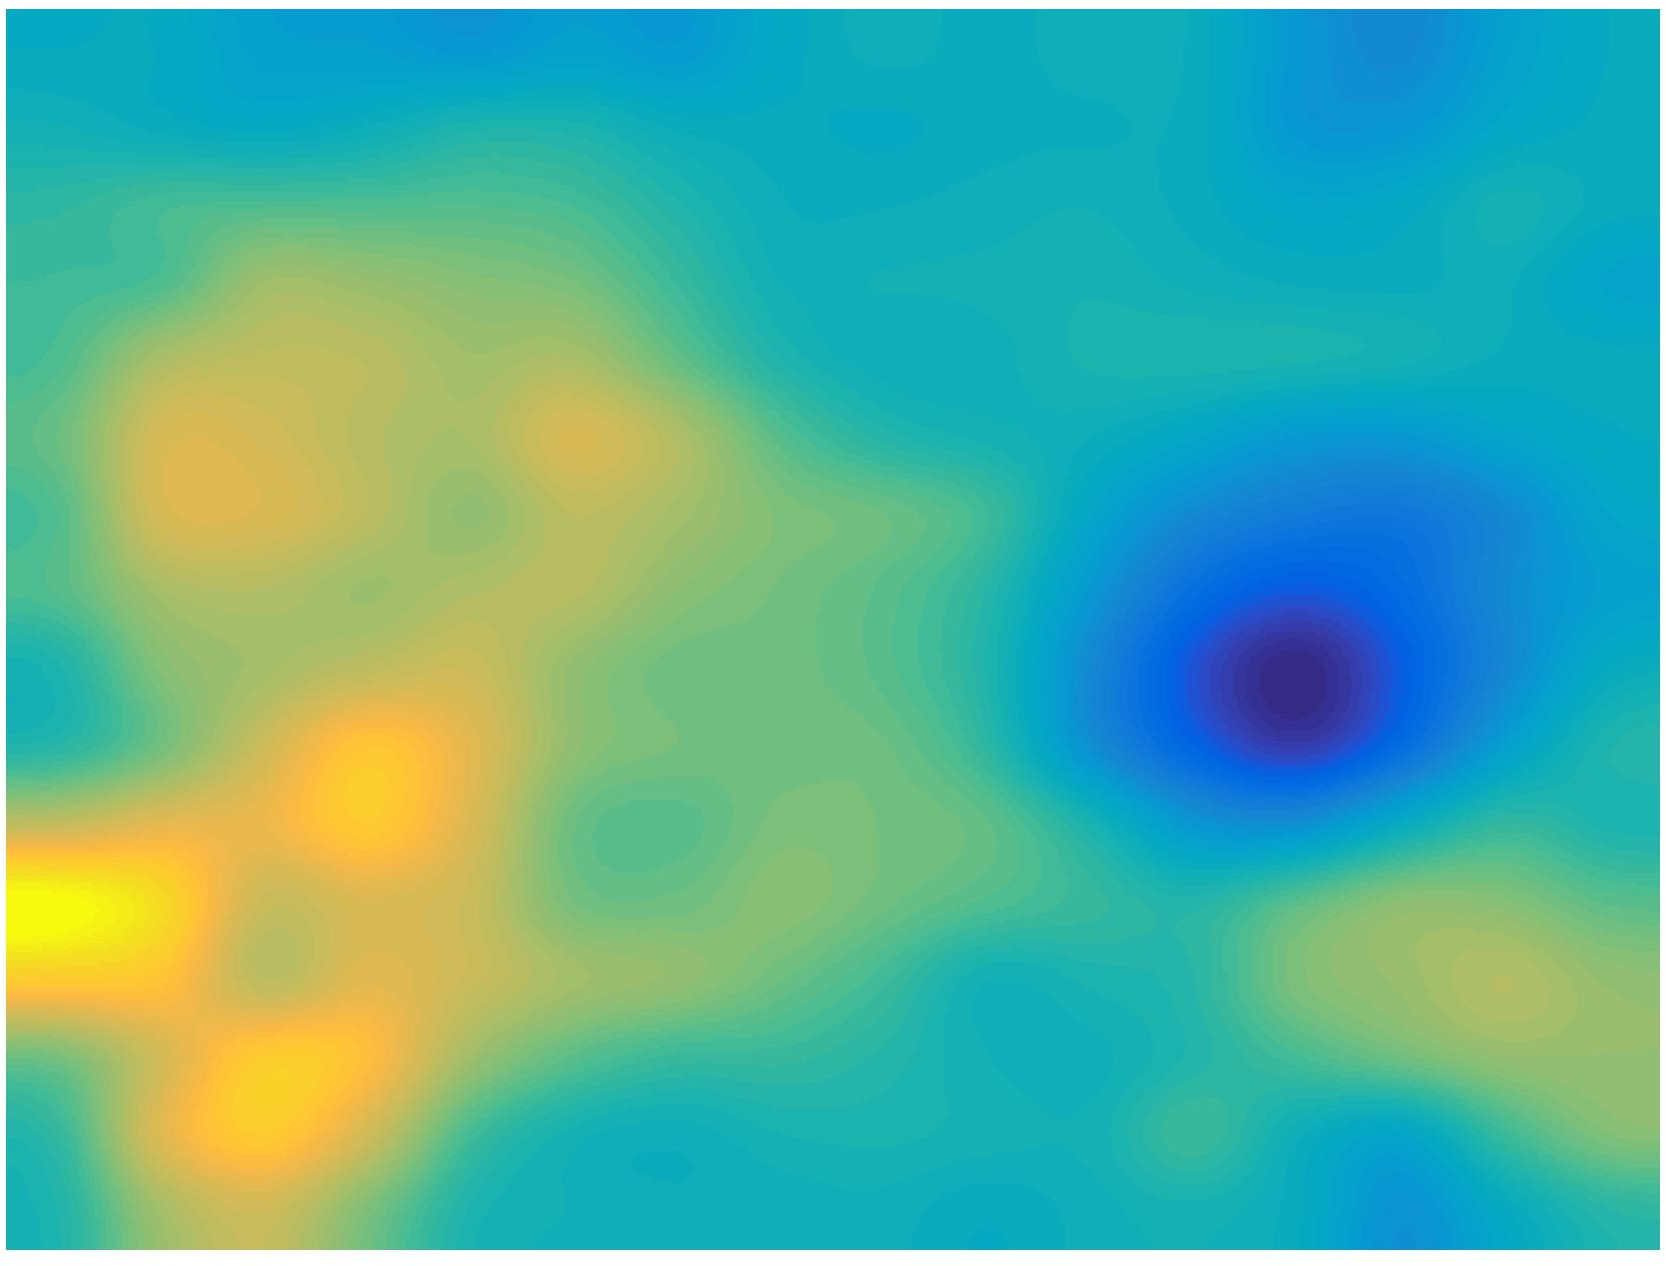
\includegraphics[width=\mapsizex cm]{images/2007_001763_dog_1}};
\node[inner sep=0pt,cm={\mapr ,0.5 ,0 ,1  ,(0 cm,0 cm)}] at (\x, \y+\mapy){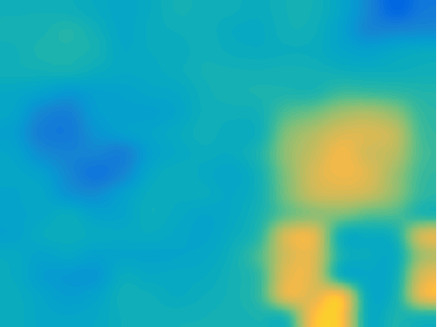
\includegraphics[width=\mapsizex cm]{images/2007_001763_cat_2}};
\node[inner sep=0pt,cm={\mapr ,0.5 ,0 ,1  ,(0 cm,0 cm)}] at (\x, \y-\mapy-\offsety){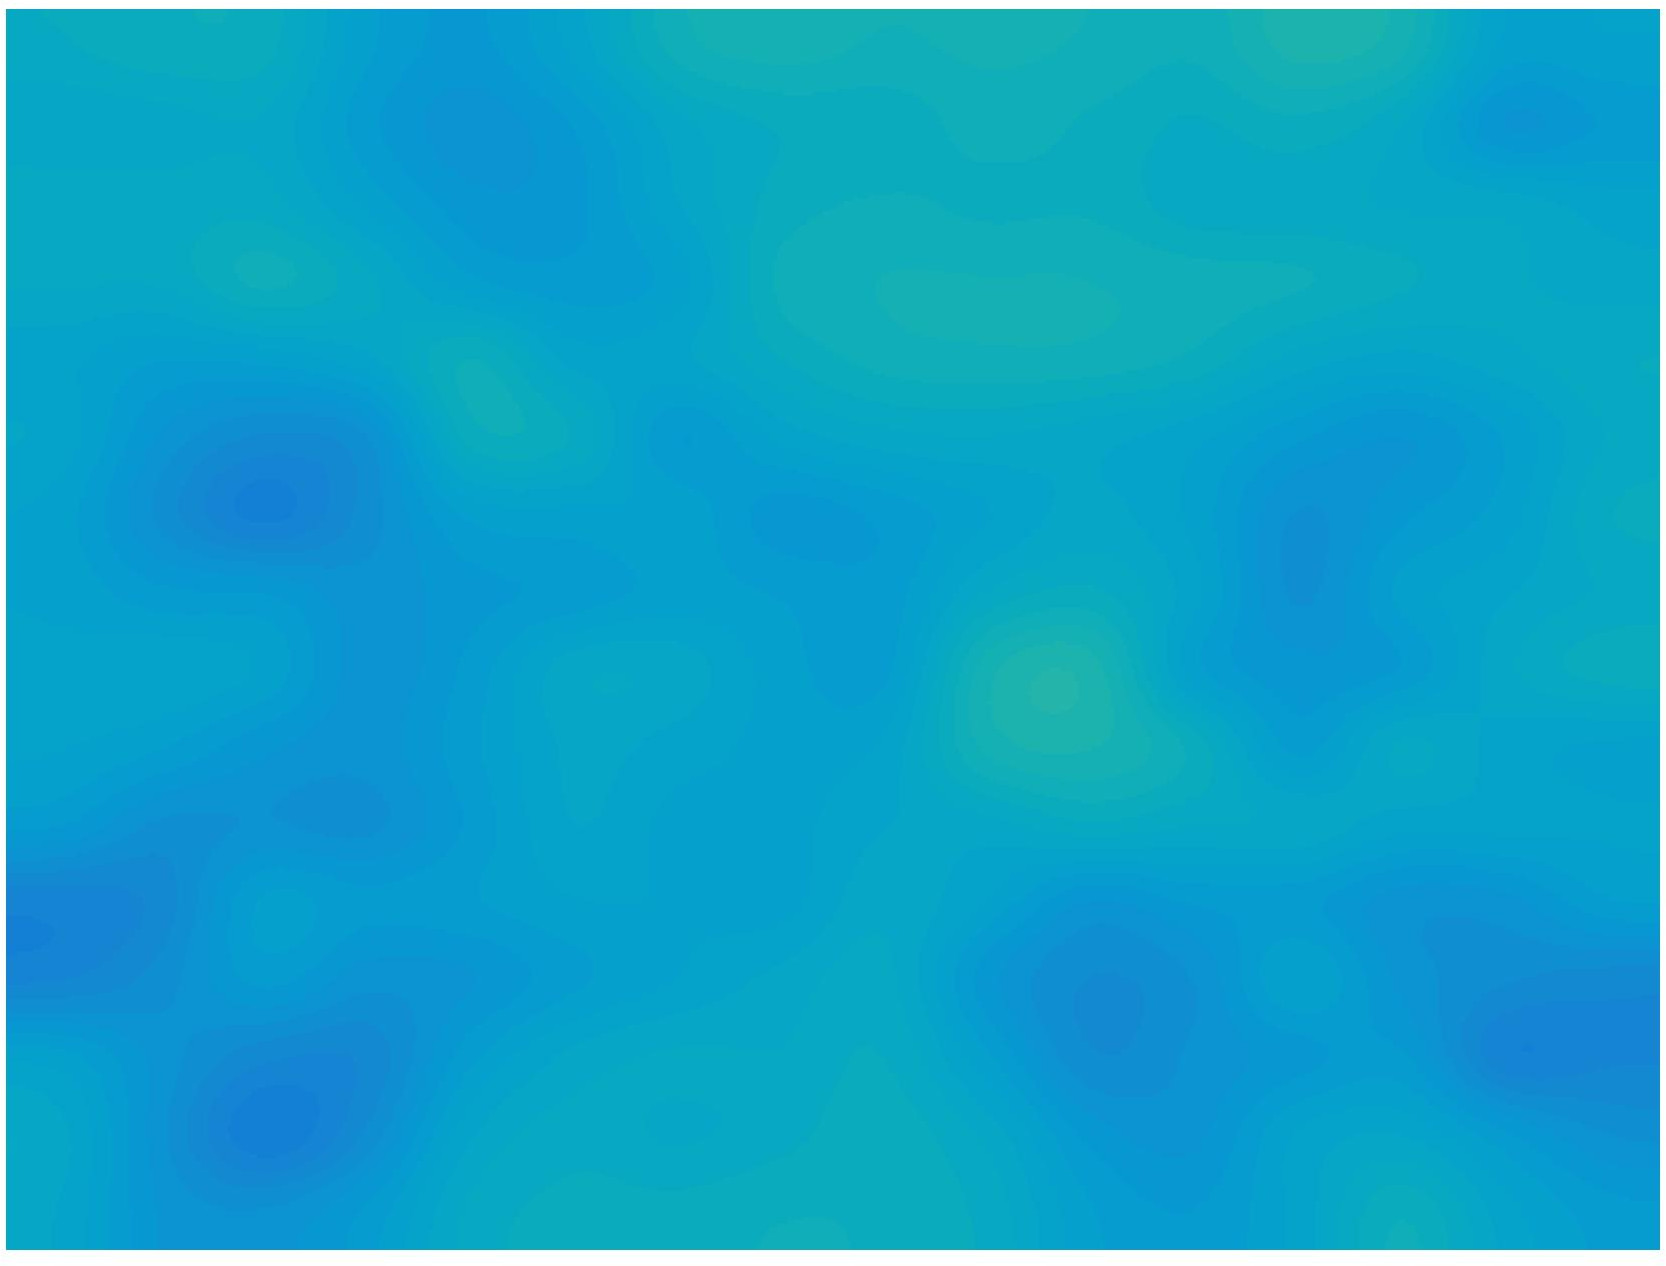
\includegraphics[width=\mapsizex cm]{images/2007_001763_train_1}};

\node (multimap1_output) at (\x+0.8, \y) {};
\node (multimap2_output) at (\x+0.8, \y+\mapy) {};
\node (multimap3_output) at (\x+0.8, \y-\mapy-\offsety) {};

% 1 map / class
\pgfmathsetmacro{\x}{\x+\offset+2}
\node[inner sep=0pt,cm={\mapr ,0.5 ,0 ,1  ,(0 cm,0 cm)}] at (\x, \y+\mapy) {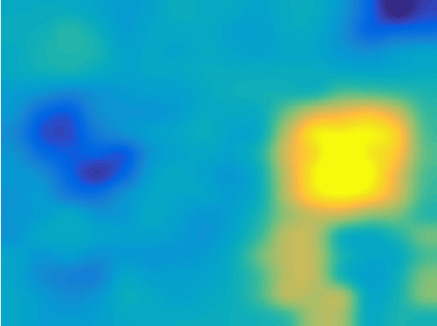
\includegraphics[width=\mapsizex cm]{images/2007_001763_cat_pool}};
\node[inner sep=0pt,cm={\mapr ,0.5 ,0 ,1  ,(0 cm,0 cm)}] at (\x, \y) {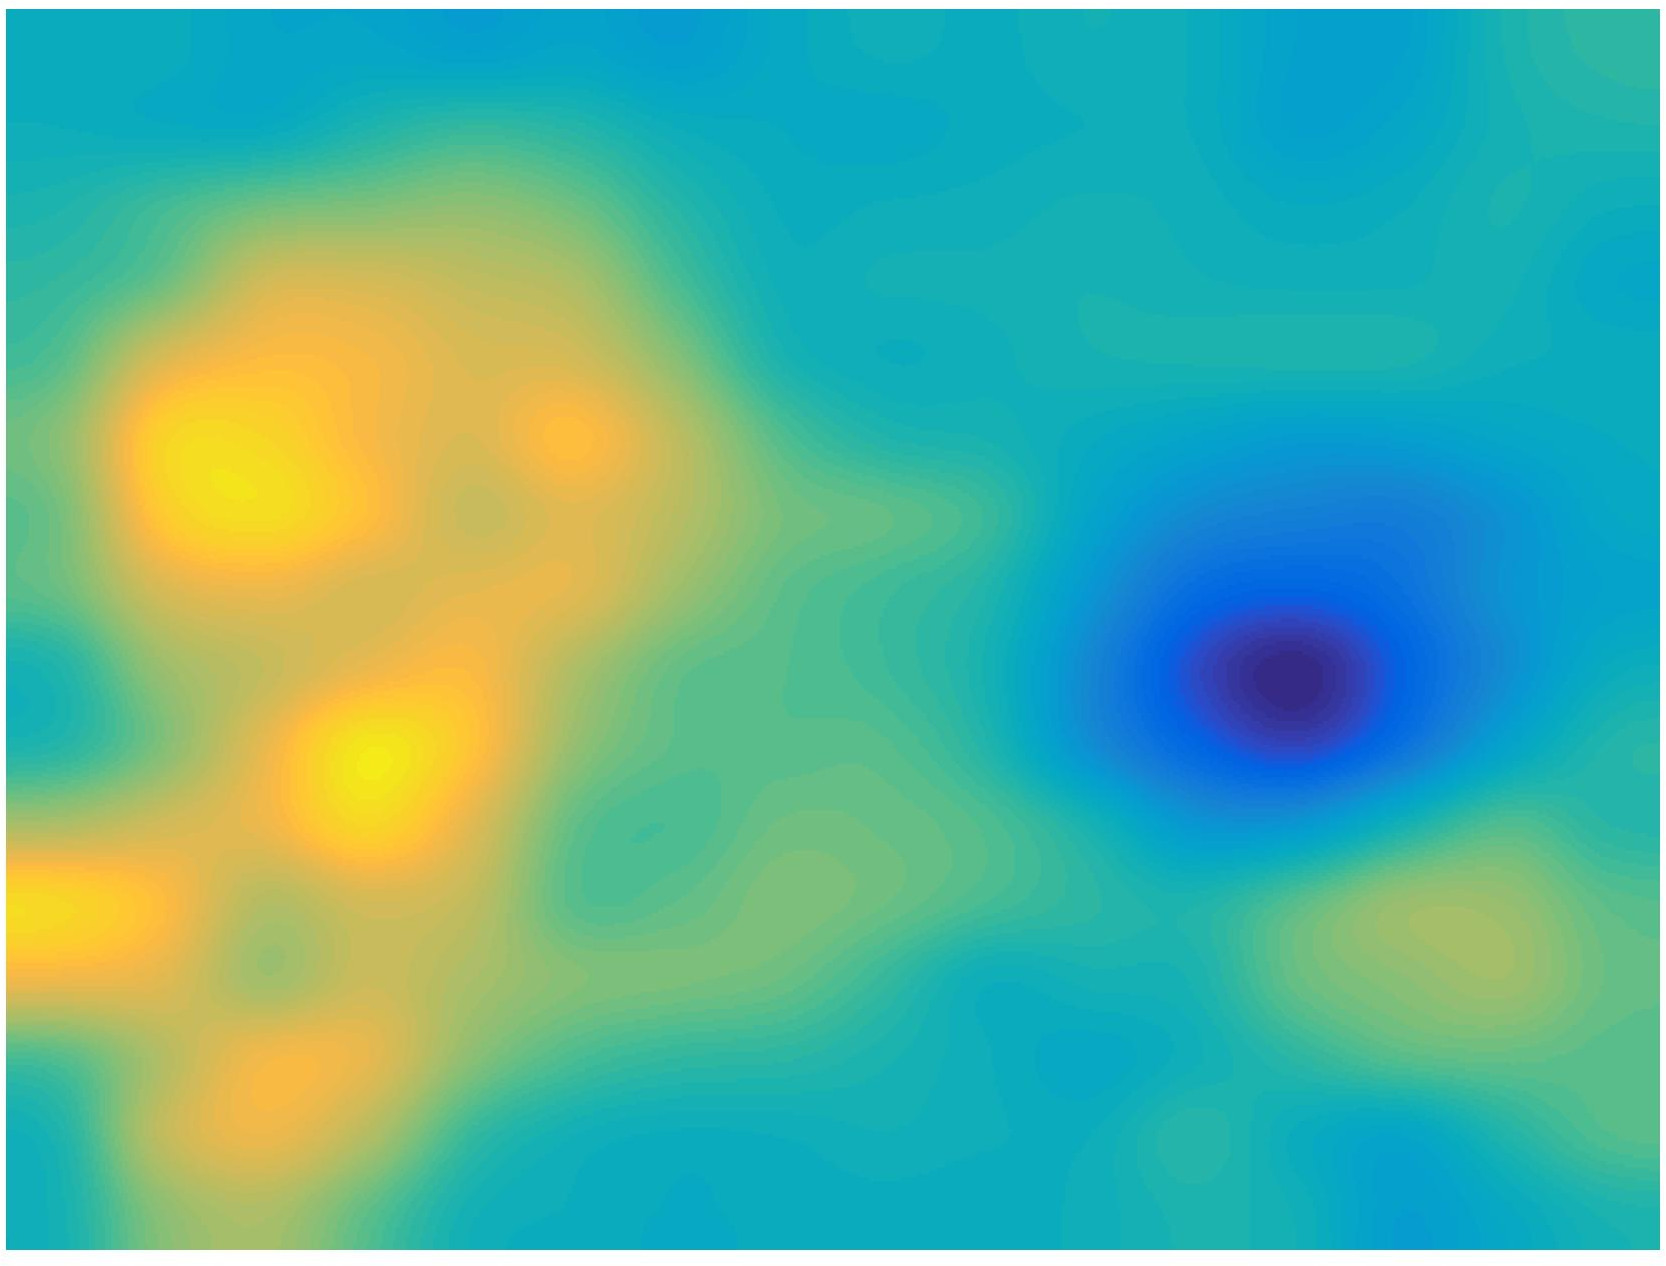
\includegraphics[width=\mapsizex cm]{images/2007_001763_dog_pool}};
\node[inner sep=0pt,cm={\mapr ,0.5 ,0 ,1  ,(0 cm,0 cm)}] at (\x, \y-\mapy-\offsety) {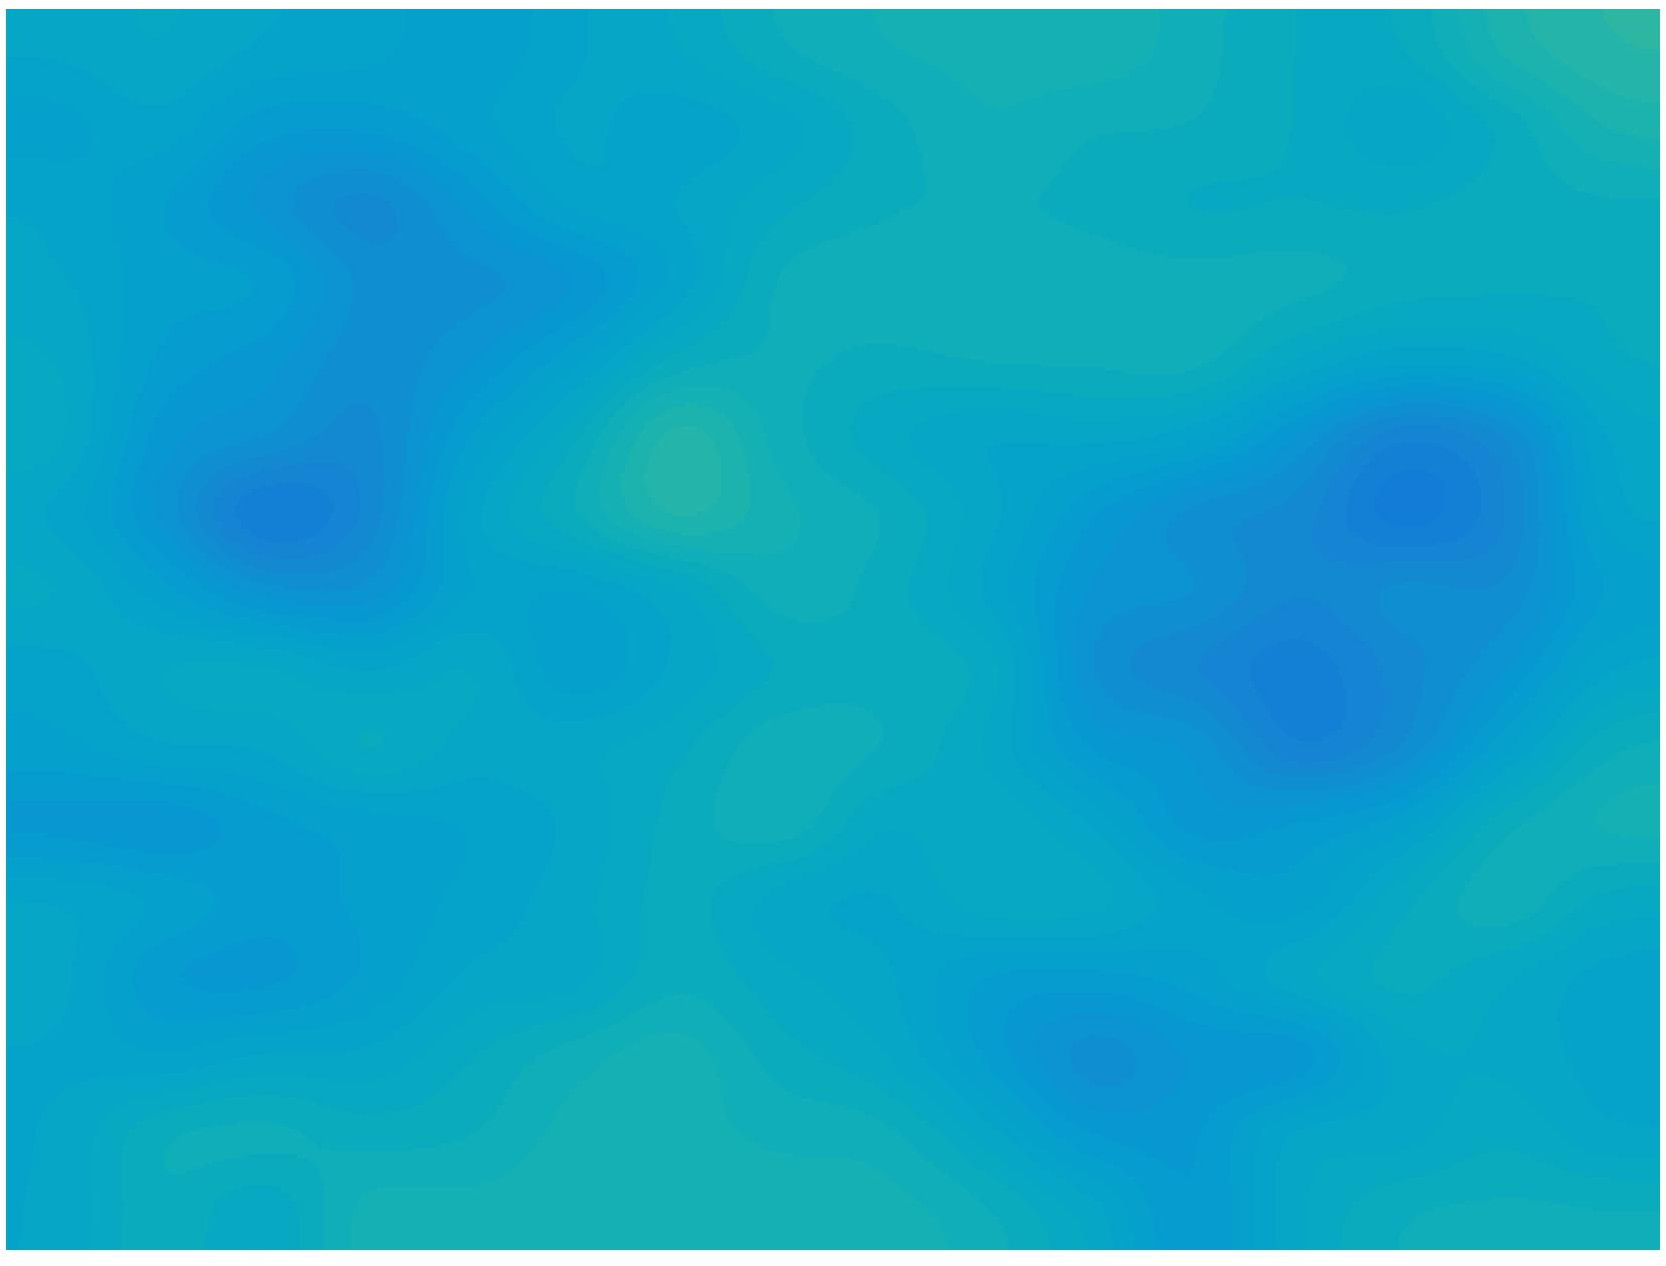
\includegraphics[width=\mapsizex cm]{images/2007_001763_train_pool}};

\node (pool1_input) at (\x-0.6, \y) {};
\node (pool2_input) at (\x-0.6, \y+\mapy) {};
\node (pool3_input) at (\x-0.6, \y-\mapy-\offsety) {};

\draw[->, line width=\linesize pt] (multimap1_output) edge (pool1_input);
\draw[->, line width=\linesize pt] (multimap2_output) edge (pool2_input);
\draw[->, line width=\linesize pt] (multimap3_output) edge (pool3_input);


\node[text width=3cm] at (\x-1.5, \y+0.7) {class-wise pooling};
\node[text width=3cm] at (\x-1.5, \y+\mapy+0.7) {class-wise pooling};
\node[text width=3cm] at (\x-1.5, \y-\mapy+0.7-\offsety) {class-wise pooling};

\node (pool1_output) at (\x+0.8, \y) {};
\node (pool2_output) at (\x+0.8, \y+\mapy) {};
\node (pool3_output) at (\x+0.8, \y-\mapy-\offsety) {};

\pgfmathsetmacro{\x}{\x+2.5}
\node[inner sep=0pt,cm={\mapr ,0.5 ,0 ,1  ,(0 cm,0 cm)}] at (\x, \y) {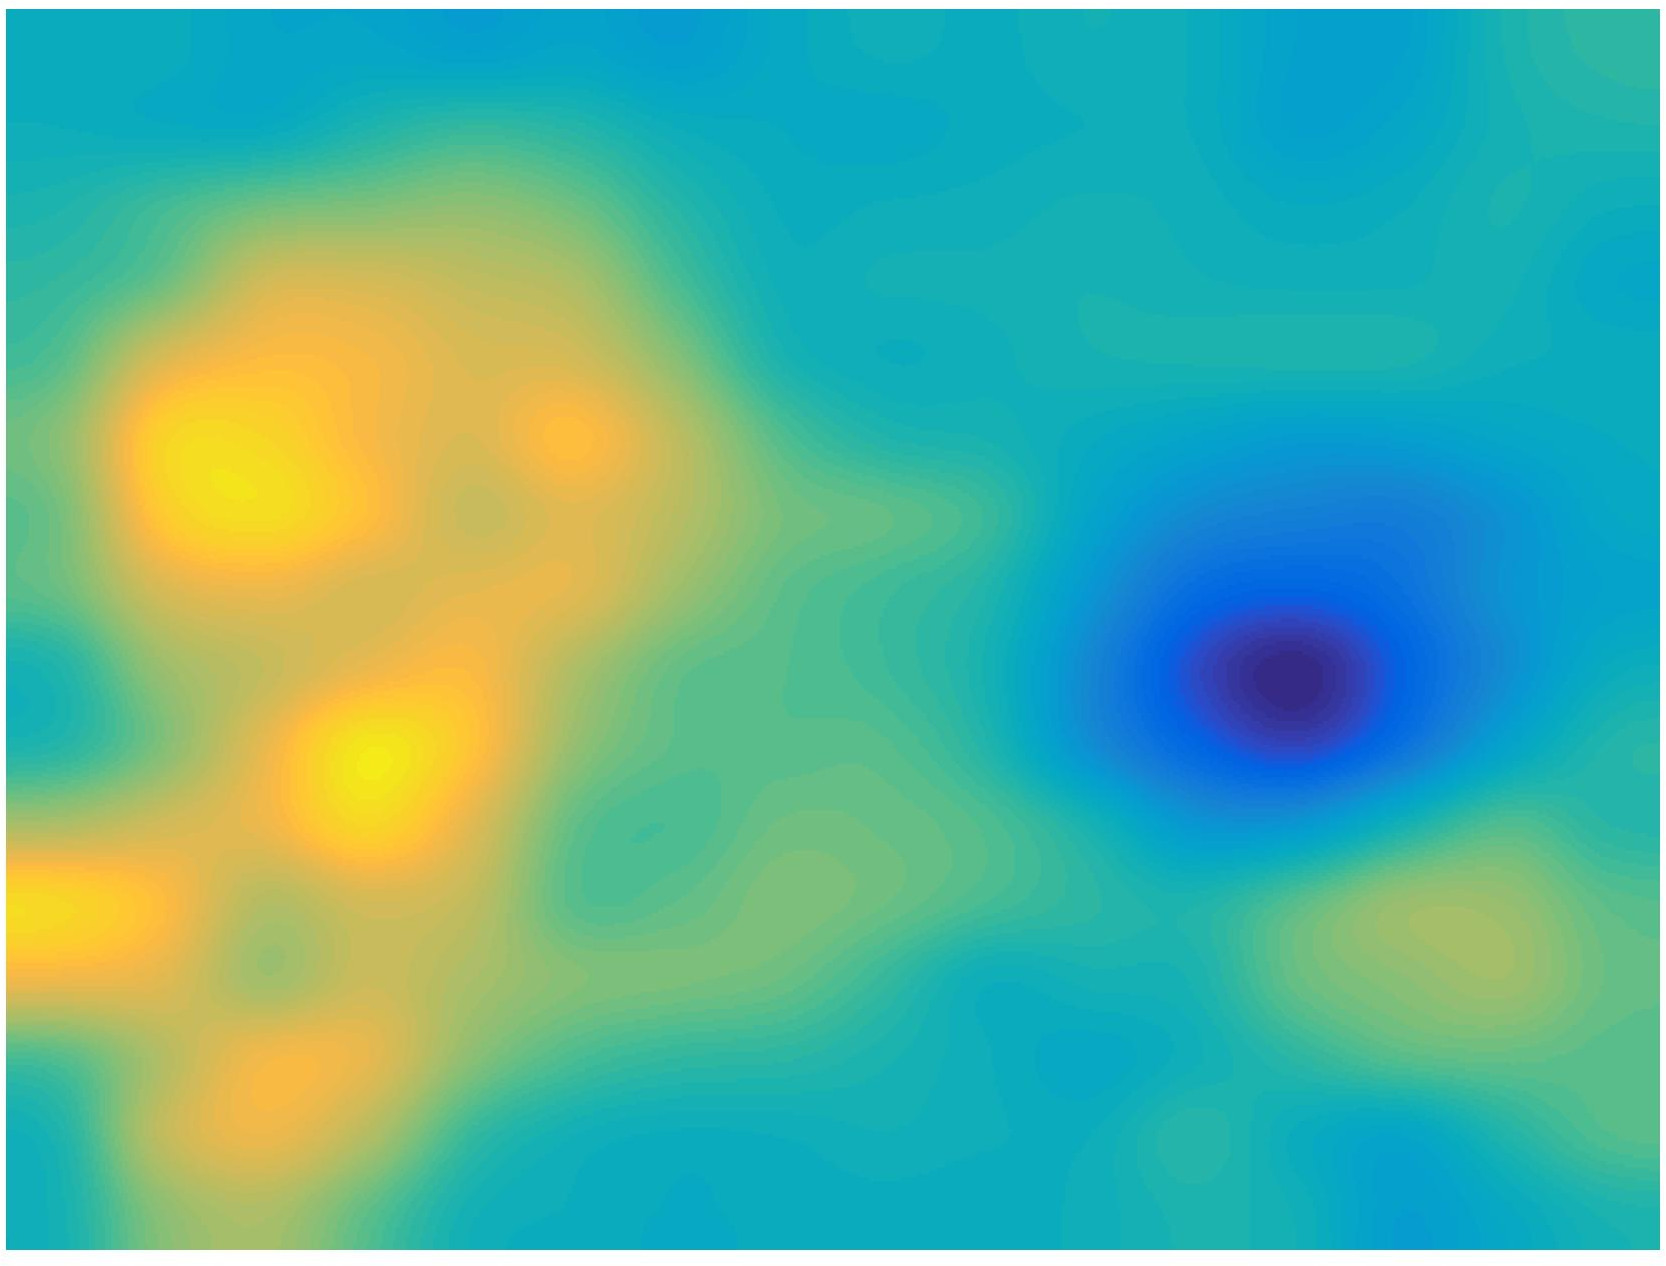
\includegraphics[width=\mapsizex cm]{images/2007_001763_dog_pool}};
\node (map1_input) at (\x-0.6, \y) {};

\pgfmathsetmacro{\x}{\x+\mapx}
\node[inner sep=0pt,cm={\mapr ,0.5 ,0 ,1  ,(0 cm,0 cm)}] at (\x, \y) {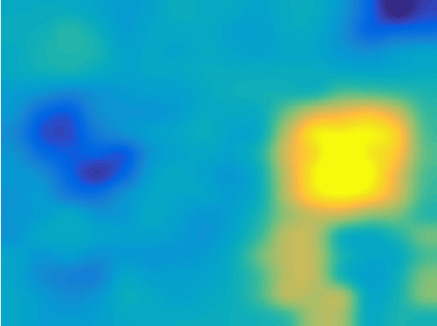
\includegraphics[width=\mapsizex cm]{images/2007_001763_cat_pool}};
\node (map2_input) at (\x+0.5,\y+1.8) {};

\pgfmathsetmacro{\x}{\x+2*\mapx}
\node at (\x-1.2,\y-1.7) {$\ldots$};
\node[inner sep=0pt,cm={\mapr ,0.5 ,0 ,1  ,(0 cm,0 cm)}] at (\x, \y) {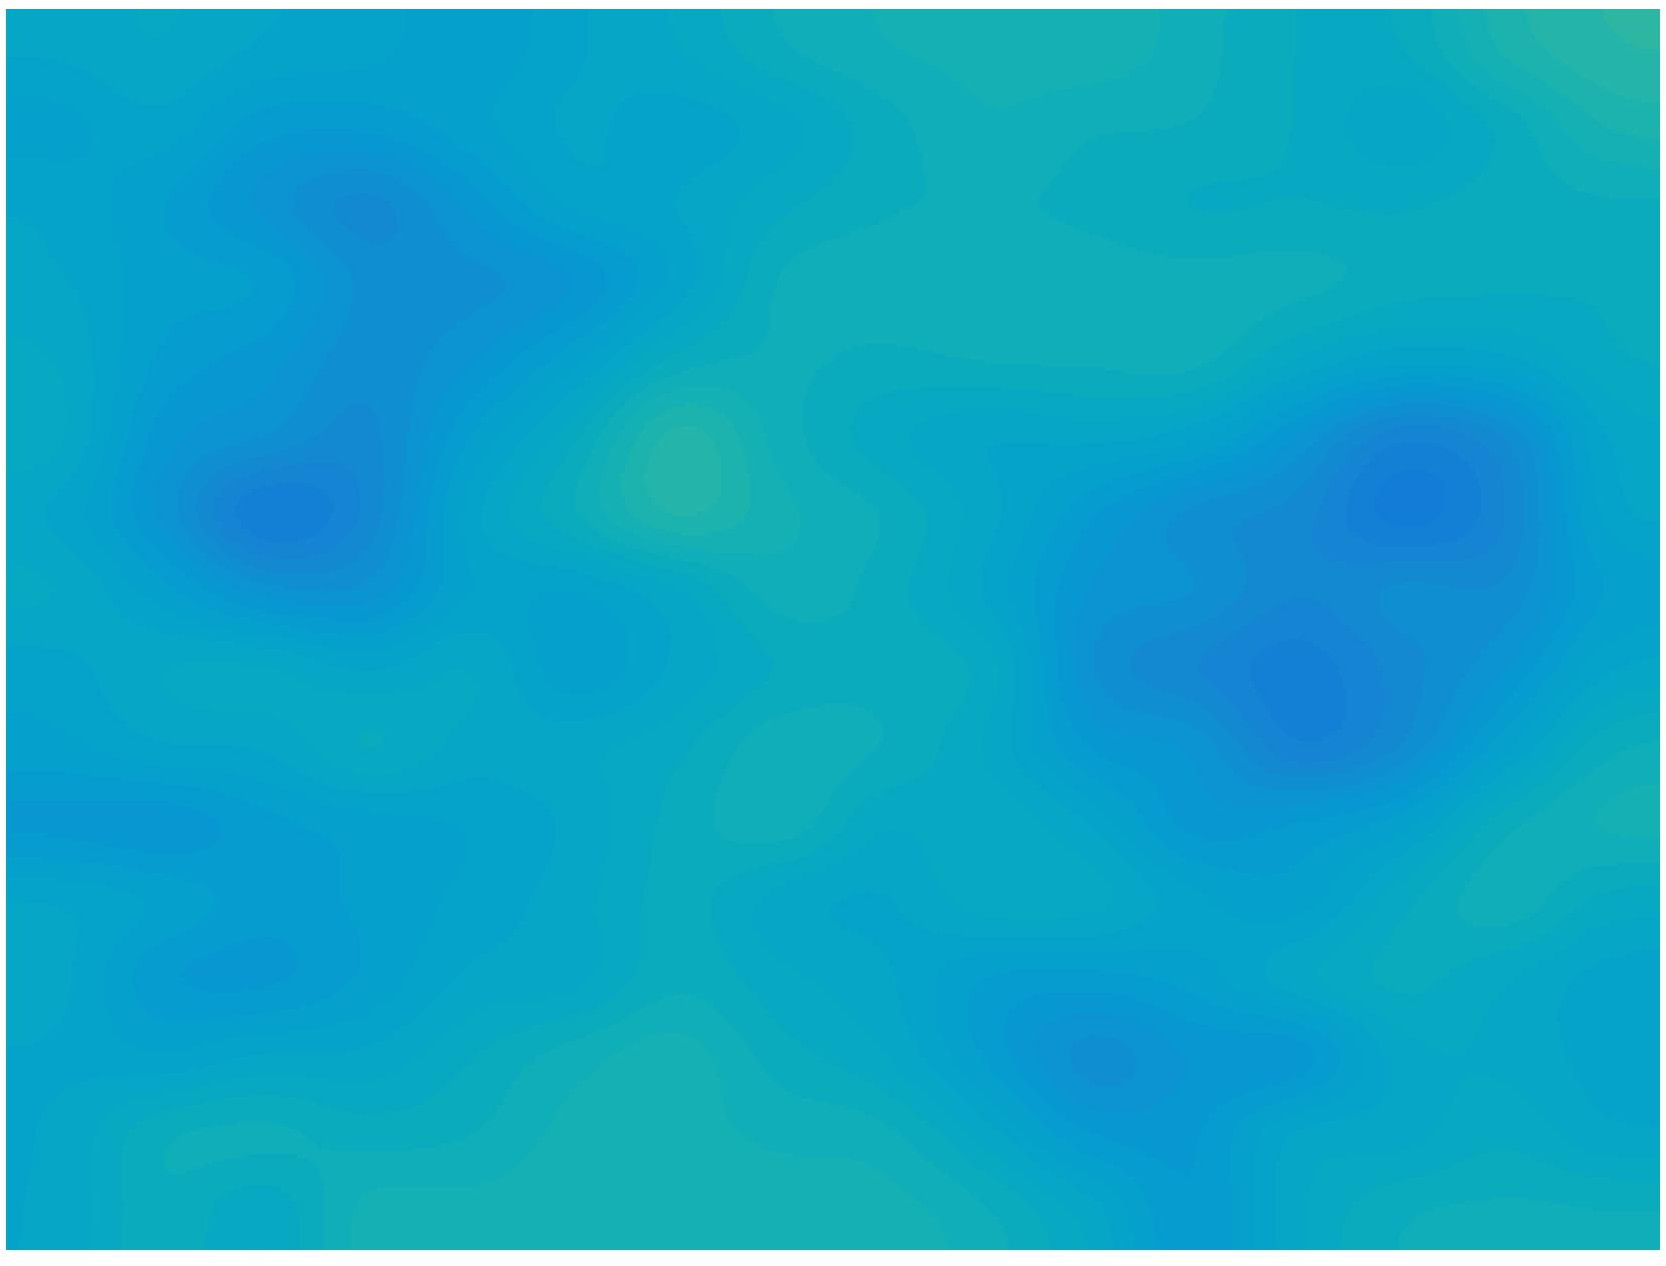
\includegraphics[width=\mapsizex cm]{images/2007_001763_train_pool}};
\node (map3_input) at (\x-0.3,\y-1.7) {};

\draw[->, line width=\linesize pt] (pool1_output) edge (map1_input);
\draw[->, line width=\linesize pt] (pool2_output) edge[out=0, in=90] (map2_input);
\draw[->, line width=\linesize pt] (pool3_output) edge[out=0, in=-90] (map3_input);

\draw [decorate,decoration={brace,amplitude=5pt,mirror,raise=4pt}, line width=\linesize pt] (\x-2.8,\y-1.8) -- (\x-0.5,\y-1.8);
\node at (\x-1.7,\y-2.5) {$C$};

\node (maps_output) at (\x+0.6, \y) {};

\pgfmathsetmacro{\x}{\x+\offset}
\node (localization) at (\x+0.5, \y) {};
\node (segmentation) at (\x+0.5, \y-\mapy) {};
\node (classification) at (\x+0.5, \y+\mapy) {};

\draw[->, line width=\linesize pt] (maps_output) edge (classification);
\draw[->, line width=\linesize pt] (maps_output) edge (localization);
\draw[->, line width=\linesize pt] (maps_output) edge (segmentation);

\node[text width=2cm] at (\x-0.5, \y+\mapy) {spatial pooling};
\pgfmathsetmacro{\x}{\x+0.5}

% orientation
\pgfmathsetmacro{\xx}{-0.02}
\pgfmathsetmacro{\cubex}{2}
\pgfmathsetmacro{\cubey}{0.25}
\pgfmathsetmacro{\cubez}{\cubey}

\pgfmathsetmacro{\xo}{\x+2.5}
\pgfmathsetmacro{\yo}{\y+\mapy + 0.5}
\draw[convline,fill=convfill, line width=\linesize pt] (\xo+\xx/2,\yo+\cubey/2,\cubez/2) -- ++(-\cubex,0,0) -- ++(0,-\cubey,0) -- ++(\cubex,0,0) -- cycle;
\draw[convline,fill=convfill, line width=\linesize pt] (\xo+\xx/2,\yo+\cubey/2,\cubez/2) -- ++(0-\xx,0,-\cubez) -- ++(0,-\cubey,0) -- ++(0+\xx,0,\cubez) -- cycle;
\draw[convline,fill=convfill, line width=\linesize pt] (\xo+\xx/2,\yo+\cubey/2,\cubez/2) -- ++(-\cubex,0,0) -- ++(0-\xx,0,-\cubez) -- ++(\cubex,0,0) -- cycle;

\node (poolc_left) at (\xo+\xx/2-\cubex-\xx-0.1,\yo + \cubey/2+0.2,\cubez/2-\cubez) {}; % invisible node
\node (poolc_right) at (\xo+\xx/2-\xx+0.1,\yo + \cubey/2+0.2,\cubez/2-\cubez) {}; % invisible node
\draw[<->, line width=\linesize pt] (poolc_left) edge (poolc_right);

\node at (\xo - \cubex/2, \yo + \cubey/2+0.5,\cubez/2-\cubez) {$C$};

\pgfmathsetmacro{\x}{\x+2}
\node at (\x+0.7, \y+6) {\textbf{Classification}};
\pgfmathsetmacro{\xo}{\xo+2.5}
\pgfmathsetmacro{\yo}{\yo+0.5*\classify}
\node[text width=3cm] at (\xo-0.2,\yo-0.5*\classify) {\textcolor{green}{\cmark} dog };
\node[text width=3cm] at (\xo-0.2,\yo+0.5*\classify) {\textcolor{green}{\cmark} cat };
\node[text width=3cm] at (\xo-0.2,\yo-1.5*\classify) {\textcolor{red}{\xmark} bus };

\pgfmathsetmacro{\imsizex}{5}
\node at (\x+0.7, \y+0.3){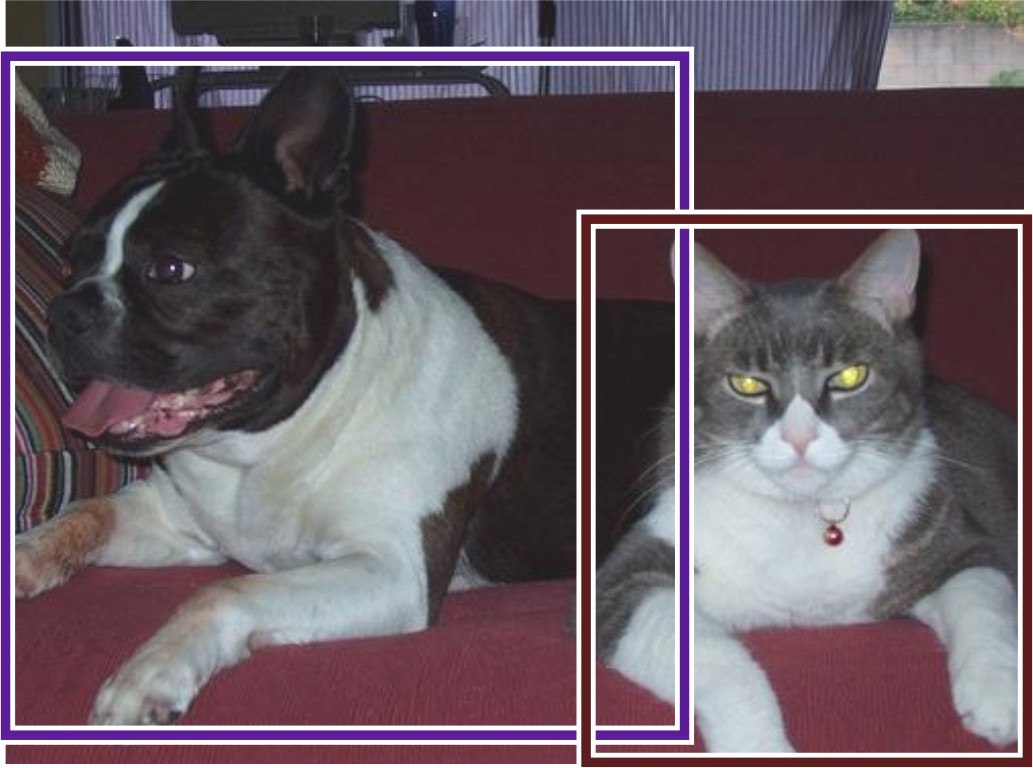
\includegraphics[width=\imsizex cm]{images/2007_001763_localization}};
\node at (\x+0.7, \y+2.5) {\textbf{Localization}};
\node at (\x+0.7, \y-4.4){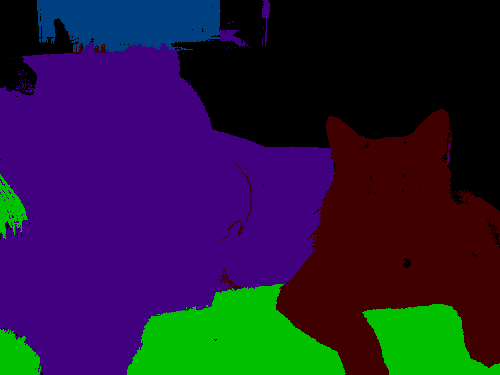
\includegraphics[width=\imsizex cm]{images/2007_001763_mask}};
\node at (\x+0.7, \y-2.2) {\textbf{Segmentation}};

\end{tikzpicture}

\end{document}